\documentclass[thesis]{subfiles}

\begin{document}

% TODO: Explain what modifications are needed to the layout tabulation and loop execution codes

\chapter{Parallelism}
\label{chapter:parallel}

Just like Firedrake (e.g.~\cite{betteridgeCodeGenerationProductive2021}) and PETSc (e.g.~???), \pyop3 is designed to be run efficiently on even the world's largest supercomputers.
Accordingly, \pyop3 is designed to work SPMD with MPI/distributed memory.
As with Firedrake and PETSc, MPI is chosen as the sole parallel abstraction; hybrid models also using shared memory libraries like OpenMP (cite) are not used because the posited performance advantages are contentious \parencite{knepleyExascaleComputingThreads2015} and would increase the complexity of the code.

\section{Message passing with star forests}

\begin{figure}
  \centering
  %
  \begin{subfigure}{\textwidth}
    \centering
    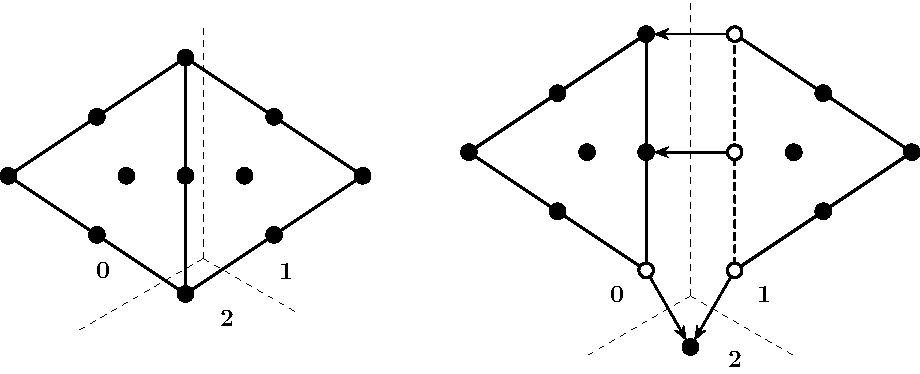
\includegraphics[width=\textwidth]{star_forest_point.pdf}
    \caption{TODO}
    \label{fig:star_forest_point}
  \end{subfigure}
  %
  \begin{subfigure}{\textwidth}
    \centering
    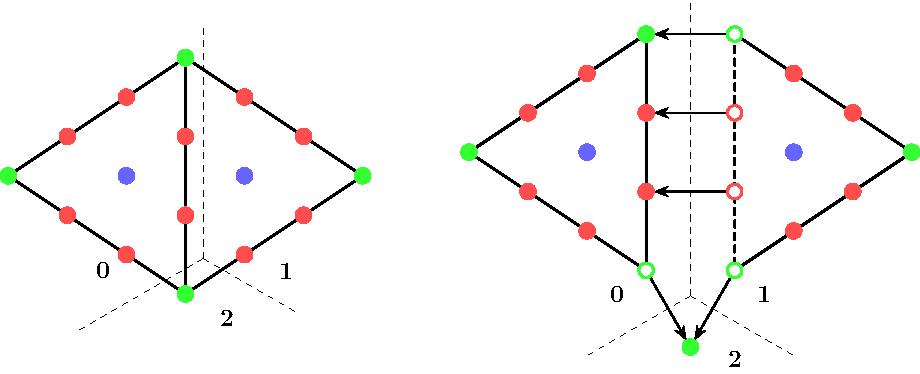
\includegraphics[width=\textwidth]{star_forest_dof.pdf}
    \caption{TODO}
    \label{fig:star_forest_dof}
  \end{subfigure}
  %
  \caption{TODO}
  \label{fig:star_forest}
\end{figure}

Almost all message passing in \pyop3 is handled by star forests, specifically by PETSc star forests (\ccode{PetscSF}) \parencite{zhangPetscSFScalableCommunication2021}.

A star forest is defined as a collection of stars, where a star is defined as a tree with a single root and potentially many leaves.
Star forests are effective for describing point-to-point MPI operations because they naturally encode the source and destination nodes as roots and leaves of the stars.
They can flexibly describe a range of different communication patterns.
% TODO ref figure
For example, a value shared globally across $n$ ranks can be represented as a star forest containing a single star with the root node on rank 0 and $n-1$ leaves, 1 for each other rank.
This is shown in Figure~\ref{fig:???}.
Star forests are also suitable for describing the overlap between parts of a distributed mesh.
In this case, each star in the forest represents a single point (cell, edge, vertex) in the mesh with the root on the ``owning" rank and leaves on the ranks where the point appears as a ``ghost".
An example of such a distribution is shown in Figure~\ref{???}.

\begin{figure}

% subfigure: global SF pattern

% 1.
% x
% 
% 2. (with arrows)
%  p0   |  p1
%    x  |   o
%      / \
%     / o \
%    /  p2 \

% subfigure: mesh-like SF pattern
% do the same thing as for globals, but use a 1-cell triangular mesh

\end{figure}

\textbf{Some terminology}

\begin{itemize}
  % these are already determined
  % \item Roots
  % \item Leaves
  \item Owned
    Points are termed ``owned" if they are present on a process and are not a leaf pointing to some other rank.
  \item Core
    Points are ``core" if they are owned \textit{and} are not part of (i.e. a root of) any star.
\end{itemize}

% need section here explaining what a halo exchange is and mesh distribution/overlap I suppose

\section{Overlapping computation and communication}

% NOTE: reference sec:pyop2_parallel. I mention that two concepts are conflated: data partitioning and iteration set partitioning.
% in pyop3 we split into owned+ghost (data) and core+noncore (iterset)

% "BUT...
% (express as a limitation, rather than a mistake.)
\begin{itemize}
  \item
    \textbf{The iteration is conflated with the data layout}\\
    ...
    For instance, it is not possible to perform parallel loops using larger stencils because the \textit{core}-\textit{owned} split is different.
    Embedding the iteration set into the data layout means that the underlying sets of the data structures are invalid.

  \item
    \textbf{The parallel decomposition is assumed to be the same for all data structures}\\
    It is not always the case that all data structures will be defined on the same mesh (e.g. mesh transfer operations).
    In such a case the algorithms used to determine \textit{core} and \textit{owned} points no longer work because the algorithm does not take into account the parallel decomposition of the other mesh.
    \textit{Core} points on one mesh may be \textit{ghost} in another, and hence the \textit{core} points ought to be labelled \textit{owned}.
\end{itemize}

These limitations suggest a new approach: the partitioning of data and the partitioning of the iteration set should be \textit{distinct processes}.
In \pyop3 we adopt the following new terminology:

\begin{itemize}
  \item
    Data structures (axis trees) are partitioned into \textit{owned} and \textit{ghost} points with all \textit{owned} points being stored contiguously before the \textit{ghost} points.

  \item
    Loop expression iteration sets are split into \textit{core} and \textit{non-core} sets.
    This partitioning is established by running over the iteration set and checking the access pattern for all arguments.
    If any of the arguments require halo data then the iteration point is classified as \textit{non-core}.
    All remaining points are then classified \textit{core}.
    %Rather than being contiguous, the indices are split into two ordered and interleaved subsets. % easy to implement!
    As ghost points are not iterated over they are not included in the subsets.
\end{itemize}

% store ghost points at the end because we need to build local vector

\begin{figure}
  \begin{subfigure}{\textwidth}
    \includegraphics{iterset_partition_cell}
    \caption{TODO}
    \label{fig:iterset_partition_cell}
  \end{subfigure}
  %
  \begin{subfigure}{\textwidth}
    \includegraphics{iterset_partition_facet}
    \caption{TODO}
    \label{fig:iterset_partition_facet}
  \end{subfigure}
  %
  \caption{TODO}
  \label{fig:iterset_partition}
\end{figure}

In order to hide the often expensive latencies associated with halo exchanges, \pyop3 uses non-blocking MPI operations to interleave computation and communication.
Since distributed meshes only need to communicate data at their boundary, and given the surface-area-to-volume ratio effect, the bulk of the required computation can happen without using any halo data.
The algorithm for overlapping computation and communication therefore looks like this:

\begin{enumerate}
  \item Initiate non-blocking halo exchanges.
  \item Compute results for data that does not rely on the completion of these halo exchanges.
  \item Block until the halo exchanges are complete.
  \item Compute results for data that requires up-to-date halo data.
\end{enumerate}

This interleaving approach is used in \pyop2 and has been reimplemented, with slight improvements, in \pyop3.

% TODO validate that these statements are correct
Although this interleaving approach may seem like the most sensible approach to this problem, it is worthwhile to note that there are subtle performance considerations that affect the effectiveness of the algorithm over a simpler blocking halo exchange approach.
\cite{bisbasAutomatedMPICode2023} showed that, in the (structured) finite difference setting, it is in fact often a better choice to use blocking exchanges because
(a) the background thread running the non-blocking communication occasionally interrupts the stream of execution, and
(b) looping over entries that touch halo data separately adversely affects data locality.
With \pyop3 we have only implemented the non-blocking approach for now, though a comparison with blocking exchanges in the context of an unstructured mesh would be interesting to pursue in future.

\subsection{Lazy communication}

Coupled with the goal of ``don't wait for data you don't need", \pyop3 also obeys the principle of ``don't send data if you don't have to".
\pyop3 associates with each parallel data structure two attributes: \pycode{leaves_valid} and \pycode{pending_reduction}.
The former tracks whether or not leaves (ghost points) contain up-to-date values.
The latter tracks, in a manner of speaking, the validity of the roots of the star forest.
If the leaves of the forest were modified, \pycode{pending_reduction} stores the reduction operation that needs to be executed for the roots of the star forest to contain correct values.
As an example, were values to be incremented into the leaves\footnote{For this to be valid the leaves need to be zeroed beforehand.}, a \ccode{SUM} reduction would be required for owned values to be synchronised.
If there is no pending reduction, the roots are considered to be valid.

The advantage to having these attributes is that they allow \pyop3 to only perform halo exchanges when absolutely necessary.
Some pertinent cases include:

\begin{itemize}
  \item If the array is being written to \pycode{op3.WRITE}, all prior writes may be discarded.
  \item If the array is being read from (\pycode{op3.READ}) and all values are already up-to-date, no exchange is necessary.
  \item If the array is being incremented into (\pycode{op3.INC}) multiple times in a row, no exchange is needed as the reductions commute.
\end{itemize}

One can further extend this by considering the access patterns of the arrays involved.
If the iteration does not touch leaves in the star forest then this affects, access descriptor dependent, whether or not certain broadcasts or reduction are required.
This is shown, alongside the rest in Algorithm~\ref{alg:???}.

% TODO show algorithm
    % def _array_updates(self):
    %     """Collect appropriate callables for updating shared values in the right order.
    %
    %     Returns
    %     -------
    %     (initializers, (finalizers0, finalizers1))
    %         Collections of callables to be executed at the right times.
    %
    %     """
    %     initializers = []
    %     finalizerss = ([], [])
    %     for array, intent, touches_ghost_points in self._distarray_args:
    %         if intent in {READ, RW}:
    %             if touches_ghost_points:
    %                 if not array._roots_valid:
    %                     initializers.append(array._reduce_leaves_to_roots_begin)
    %                     finalizerss[0].extend(
    %                         [
    %                             array._reduce_leaves_to_roots_end,
    %                             array._broadcast_roots_to_leaves_begin,
    %                         ]
    %                     )
    %                     finalizerss[1].append(array._broadcast_roots_to_leaves_end)
    %                 else:
    %                     initializers.append(array._broadcast_roots_to_leaves_begin)
    %                     finalizerss[1].append(array._broadcast_roots_to_leaves_end)
    %             else:
    %                 if not array._roots_valid:
    %                     initializers.append(array._reduce_leaves_to_roots_begin)
    %                     finalizerss[0].append(array._reduce_leaves_to_roots_end)
    %
    %         elif intent == WRITE:
    %             # Assumes that all points are written to (i.e. not a subset). If
    %             # this is not the case then a manual reduction is needed.
    %             array._leaves_valid = False
    %             array._pending_reduction = None
    %
    %         elif intent in {INC, MIN_WRITE, MIN_RW, MAX_WRITE, MAX_RW}:  # reductions
    %             # We don't need to update roots if performing the same reduction
    %             # again. For example we can increment into an array as many times
    %             # as we want. The reduction only needs to be done when the
    %             # data is read.
    %             if array._roots_valid or intent == array._pending_reduction:
    %                 pass
    %             else:
    %                 # We assume that all points are visited, and therefore that
    %                 # WRITE accesses do not need to update roots. If only a subset
    %                 # of entities are written to then a manual reduction is required.
    %                 # This is the same assumption that we make for data_wo and is
    %                 # explained in the documentation.
    %                 if intent in {INC, MIN_RW, MAX_RW}:
    %                     assert array._pending_reduction is not None
    %                     initializers.append(array._reduce_leaves_to_roots_begin)
    %                     finalizerss[0].append(array._reduce_leaves_to_roots_end)
    %
    %             # We are modifying owned values so the leaves must now be wrong
    %             array._leaves_valid = False
    %
    %             # If ghost points are not modified then no future reduction is required
    %             if not touches_ghost_points:
    %                 array._pending_reduction = None
    %             else:
    %                 array._pending_reduction = intent
    %
    %                 # set leaves to appropriate nil value
    %                 if intent == INC:
    %                     array._data[array.sf.ileaf] = 0
    %                 elif intent in {MIN_WRITE, MIN_RW}:
    %                     array._data[array.sf.ileaf] = dtype_limits(array.dtype).max
    %                 elif intent in {MAX_WRITE, MAX_RW}:
    %                     array._data[array.sf.ileaf] = dtype_limits(array.dtype).min
    %                 else:
    %                     raise AssertionError
    %
    %         else:
    %             raise AssertionError
    %
    %     return initializers, finalizerss

% where does this comment live? I like it at the end
\pyop2 is able to track leaf validity, but does not have a transparent solution for commuting reductions.

% --------------------------------------------------------------------------------

\section{Performance results}

% show some simple scaling data

\end{document}
